%%%%%%%%%%%%%%%%%%%%%%%%%%%%%%%%%%%%%%%%%%%%%%%%%%%%%%%%%%%%%%%%%%%%
\begin{frame}[c]{Who are we?}
    \setfontsize{9}
    \begin{columns}[c]
    	\begin{column}{0.3\textwidth}
    		\centering
    		\begin{tikzpicture}
    			\node[circle, minimum size=2cm, path picture={\node at (path picture bounding box.center){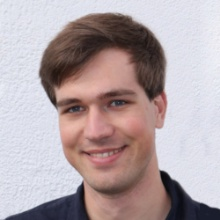
\includegraphics[height=2cm]{figures/speaker/AlexanderVanCraen}};}] {};
    		\end{tikzpicture} \\
    		\textbf{Alexander Van Craen} \\[.4em]
    		\href{mailto:Alexander.Van-Craen@ipvs.uni-stuttgart.de}{Alexander.Van-Craen@ipvs.uni-stuttgart.de}
    	\end{column}
    	\begin{column}{0.3\textwidth}
    		\centering
    		\begin{tikzpicture}
    			\node[circle,minimum size=2cm, path picture={\node at (path picture bounding box.center){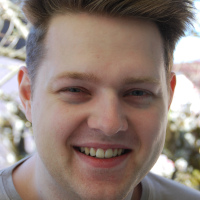
\includegraphics[height=2cm]{figures/speaker/MarcelBreyer}};}] {};
    		\end{tikzpicture} \\
    		\textbf{Marcel Breyer} \\[.4em]
    		\href{mailto:Marcel.Breyer@ipvs.uni-stuttgart.de}{Marcel.Breyer@ipvs.uni-stuttgart.de}
    	\end{column}
    	\begin{column}{0.3\textwidth}
    		\centering
    		\begin{tikzpicture}
    			\node[circle,minimum size=2cm, path picture={\node at (path picture bounding box.center){
\includegraphics[height=2cm]{figures/speaker/LinusBantel}};}] {};
    		\end{tikzpicture} \\
    		\textbf{Linus Bantel} \\[.4em]
    		\href{mailto:Linus.Bantel@ipvs.uni-stuttgart.de}{Linus.Bantel@ipvs.uni-stuttgart.de}
    	\end{column}
    \end{columns}
    \vspace*{1.5em}
    \begin{columns}
    	\begin{column}{0.3\textwidth}
    		\centering
    		\begin{tikzpicture}
    			\node[circle,minimum size=2cm, path picture={\node at (path picture bounding box.center){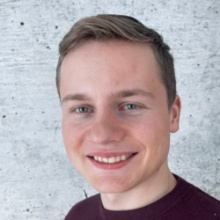
\includegraphics[height=2cm]{figures/speaker/AlexanderStrack}};}] {};
    		\end{tikzpicture} \\
    		\textbf{Alexander Strack} \\[.4em]
    		\href{mailto:Alexander.Strack@ipvs.uni-stuttgart.de}{Alexander.Strack@ipvs.uni-stuttgart.de}
    	\end{column}
    	\begin{column}{0.3\textwidth}
    		\centering
    		\begin{tikzpicture}
    			\node[circle,minimum size=2cm, path picture={\node at (path picture bounding box.center){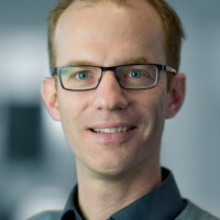
\includegraphics[height=2cm]{figures/speaker/DirkPflueger}};}] {};
    		\end{tikzpicture} \\
    		\textbf{Prof. Dr. Dirk Pflüger} \\[.4em]
    		\href{mailto:Dirk.Pflueger@ipvs.uni-stuttgart.de}{Dirk.Pflueger@ipvs.uni-stuttgart.de}
    	\end{column}
    \end{columns}
\end{frame}
%%%%%%%%%%%%%%%%%%%%%%%%%%%%%%%%%%%%%%%%%%%%%%%%%%%%%%%%%%%%%%%%%%%%

%%%%%%%%%%%%%%%%%%%%%%%%%%%%%%%%%%%%%%%%%%%%%%%%%%%%%%%%%%%%%%%%%%%%
\begin{frame}
	\frametitle{Target - Phase 1}
	\vspace*{-1.5em}
	\begin{center}
Simulation of two colliding galaxies.
	\end{center}
	\begin{figure}
		\hspace*{-.8em}
		\centering
		\BeforeAfterImage[.45]{figures/20000_300_1000000_1_1-2_0.png}
		\hspace{.5em}
		\DisplayRightArrow
		\hspace{.5em}
		\BeforeAfterImage[.48]{figures/hubble_whirpool_galaxy.jpg}
	\end{figure}
	\begin{tikzpicture}[overlay]
\node[text width=6.8cm, align=left, execute at begin node=\setlength{\baselineskip}{6pt}] at (10.8, -.4) {\scriptsize Image of the Whirlpool Galaxy (M51), located 23 million light-years away from Earth, captured by the Hubble Space Telescope in 2005.\\[.2em]\setfontsize{4pt} Source: \url{https://hubblesite.org/contents/media/images/2005/12/1677-Image.html}};
	\end{tikzpicture}
	\vfill
\end{frame}
%%%%%%%%%%%%%%%%%%%%%%%%%%%%%%%%%%%%%%%%%%%%%%%%%%%%%%%%%%%%%%%%%%%%

%%%%%%%%%%%%%%%%%%%%%%%%%%%%%%%%%%%%%%%%%%%%%%%%%%%%%%%%%%%%%%%%%%%%
\begin{frame}
	\frametitle{Target - Phase 2}
	\vspace*{-1em}
	\begin{center}
Simulation of the collision between the Milky Way and the Andromeda Galaxy.
	\end{center}
  \begin{figure}
      \centering
      \BeforeAfterImage[.45]{figures/dubinski_0-03_120_1_1-5_0.png}
      \hspace{.5em}
      \DisplayRightArrow
      \hspace{.5em}
      \BeforeAfterImage[.45]{figures/dubinski_0-03_120_1_1-5_120.png}
  \end{figure}

  \begin{tikzpicture}[overlay]
    \node[white] at (2, 4.75) {\footnotesize Andromeda};
    \node[white] at (4.7, 1.75) {\footnotesize Milky Way};
  \end{tikzpicture}
  \vfill
\end{frame}
%%%%%%%%%%%%%%%%%%%%%%%%%%%%%%%%%%%%%%%%%%%%%%%%%%%%%%%%%%%%%%%%%%%%

%%%%%%%%%%%%%%%%%%%%%%%%%%%%%%%%%%%%%%%%%%%%%%%%%%%%%%%%%%%%%%%%%%%%
\begin{frame}
  \frametitle{Learning Objectives}
  \begin{itemize}
    \item Implementation of a non-trivial project in a small group.
    \item Developing a sense for different algorithmic complexities.
    \item Practical application of tree data structures.
    \item Possible programming languages: \texttt{C++} (recommended) or \texttt{Java}.
    \item Gaining experience with \link{https://github.tik.uni-stuttgart.de/}{Git}.
    \item Familiarization with working on remote systems using the \link{www.bw-cloud.org}{bwCloud}.
    \item Utilizing established programs in scientific computing (e.g., \link{https://www.paraview.org/}{ParaView} for visualization).
  \end{itemize}
\end{frame}
%%%%%%%%%%%%%%%%%%%%%%%%%%%%%%%%%%%%%%%%%%%%%%%%%%%%%%%%%%%%%%%%%%%%

%%%%%%%%%%%%%%%%%%%%%%%%%%%%%%%%%%%%%%%%%%%%%%%%%%%%%%%%%%%%%%%%%%%%
\begin{frame}{Learning Objectives - Working Method}
\centering
{\Large\textbf{Independent Work!}}

\vfill
\pause
\textit{\enquote{%
    Manchmal hat man sich schon etwas verloren gefühlt, z.B. hatte ich 0\% Plan wie man die BW Cloud benutzt. Hab mir dann mit ganz viel Hilfe von Google und YouTube eine eigene VM aufgesetzt (ca. 10h bis alles läuft, da ich keine Vorerfahrung hatte). Es waren oft Kleinigkeiten, wo einem oft nur Foreneinträge geholfen haben (z.B. wie führe ich mit Maven in der Konsole aus, wie gebe ich Maven mehr RAM, usw.) $\dots$%
}}

\vfill
%\pause

%6 ECTS $\approx \SI{180}{\hour} \approx \num{4.5}$ Arbeitswochen à $\SI{40}{\hour}$
\end{frame}
%%%%%%%%%%%%%%%%%%%%%%%%%%%%%%%%%%%%%%%%%%%%%%%%%%%%%%%%%%%%%%%%%%%%

%%%%%%%%%%%%%%%%%%%%%%%%%%%%%%%%%%%%%%%%%%%%%%%%%%%%%%%%%%%%%%%%%%%%
\begin{frame}
  \frametitle{Procedure}
  \vspace*{-1em}
  \begin{itemize}
    \item Multiple phases:
          \begin{description}
            \item[Phase 0] Formation of groups of 3. \\
            (Deadline: \textbf{\dateDeadlinePhaseZero})
            \item[Phase 1] Familiarization with the n-body problem and implementation using the naive algorithm, including visualization. \\
            (Deadline: \textbf{\dateDeadlinePhaseOne})
            \item[Phase 2] Implementation of the tree-based Barnes-Hut algorithm, including evaluation and performance comparison with the naive algorithm. \\
            (Deadline: \textbf{\dateDeadlinePhaseTwo})
            \item[Presentation] \SI{5}{\minute} final presentation per group. \\
            (Date: \textbf{\dateFinal})
          \end{description}\pause
    \item Acceptance by the end of each phase. \\
          $\rightarrow$ Progress to the next phase only after successful acceptance of the current phase.
    \item Additionally, there is a small competition to \link{\urlNextcloud}{determine the fastest simulation}. The winners will receive a small prize.
  \end{itemize}
\end{frame}
%%%%%%%%%%%%%%%%%%%%%%%%%%%%%%%%%%%%%%%%%%%%%%%%%%%%%%%%%%%%%%%%%%%%

%%%%%%%%%%%%%%%%%%%%%%%%%%%%%%%%%%%%%%%%%%%%%%%%%%%%%%%%%%%%%%%%%%%%
\begin{frame}
  \frametitle{General - TIK GitHub}
  \begin{itemize}
    \item Mandatory use of the University's provided \link{https://github.tik.uni-stuttgart.de/}{GitHub instance} by TiK.
    \item Each student can log in with their \texttt{stXXXXXX} credentials.
    \item Create \textbf{one private} repository per submission group.
    \item Add all group members and supervisors (\supervisorAc) to the repository.
    \item Each repository \textbf{must} contain a \texttt{README} with all necessary information for compiling and running the code.
    \item \texttt{C++ + CMake} \link{https://github.com/SCTeaching-NBody/ProgrammingProject_Cpp_Template}{Repository Template}.
    \item \texttt{Java + Maven} \link{https://github.com/SCTeaching-NBody/ProgrammingProject_Java_Template}{Repository Template}.
    \url{}
    \item For a brief Git introduction, see \link{https://githowto.com/}{Git HowTo}.
  \end{itemize}
\end{frame}
%%%%%%%%%%%%%%%%%%%%%%%%%%%%%%%%%%%%%%%%%%%%%%%%%%%%%%%%%%%%%%%%%%%%

%%%%%%%%%%%%%%%%%%%%%%%%%%%%%%%%%%%%%%%%%%%%%%%%%%%%%%%%%%%%%%%%%%%%
\begin{frame}
  \frametitle{General - bwCloud}
  \begin{itemize}
    \item \link{https://www.bw-cloud.org/}{bwCloud} as the online VM hosting service of the state of Baden-Württemberg.
    \item Register: \url{https://www.bw-cloud.org/de/erste_schritte\#step1}
    \item Log in after registration: \url{https://portal.bw-cloud.org/auth/login/} (via \enquote{bwIDM via OpenID Connect} $\rightarrow$ regular st-account)
    \item Create an instance with the following configuration:
    \begin{itemize}
        \item Details: Assign a name
        \item Source: Ubuntu 22.04
        \item Flavor: m1.tiny (1 VCPU, \SI{1}{\giga\byte} RAM)
        \item Key Pair: Add your own public SSH key (Instructions for creating an SSH key on Linux or Windows: \url{https://docs.oracle.com/en/cloud/cloud-at-customer/occ-get-started/generate-ssh-key-pair.html})
    \end{itemize}
    \item Log in to the instance: \texttt{ssh ubuntu@IP\_address\_of\_the\_instance}
  \end{itemize}
\end{frame}
%%%%%%%%%%%%%%%%%%%%%%%%%%%%%%%%%%%%%%%%%%%%%%%%%%%%%%%%%%%%%%%%%%%%

%%%%%%%%%%%%%%%%%%%%%%%%%%%%%%%%%%%%%%%%%%%%%%%%%%%%%%%%%%%%%%%%%%%%
\begin{frame}[fragile]
  \frametitle{General - bwCloud: Installation of allowed software}
    \begin{itemize}
        \item Update: \mintinline{bash}{sudo apt update && sudo apt upgrade} \vspace{.5em}

        \item Allowed software for \texttt{C++}:\vspace*{-.2em}
        \begin{minted}{bash}
sudo apt install g++ cmake cmake-curses-gui
        \end{minted}

        \pause
        \item Allowed software for \texttt{Java}:\vspace*{-.2em}
        \begin{minted}[breaklines=true]{bash}
sudo apt install openjdk-18-jdk openjdk-18-jre maven
        \end{minted}
    \end{itemize}
    \vfill
    In your code, \textbf{only} the respective standard libraries (everything in \texttt{std} in \texttt{C++}, except C standard header and their \texttt{C++} counterparts (e.g., \mintinline{c++}{<string>} is allowed, \mintinline{c++}{<cstring>} or \mintinline{c++}{<string.h>} is \textbf{not} allowed), and everything in \texttt{java.*} in \texttt{Java}) may be used!
\end{frame}
%%%%%%%%%%%%%%%%%%%%%%%%%%%%%%%%%%%%%%%%%%%%%%%%%%%%%%%%%%%%%%%%%%%%

%%%%%%%%%%%%%%%%%%%%%%%%%%%%%%%%%%%%%%%%%%%%%%%%%%%%%%%%%%%%%%%%%%%%
\begin{frame}[fragile]
  \frametitle{General - ParaView}
  \vspace*{-1em}
\begin{columns}[t]
  \hspace*{2em}
  \begin{column}{.37\textwidth}
    \textcolor{beamer@blendedblue}{1.} Open simulation file:\\
    \hspace{.9em} File $\rightarrow$ Open $\rightarrow$ \texttt{.pvd} \\

    \textcolor{beamer@blendedblue}{2.} Display simulation: \\[.1em]
    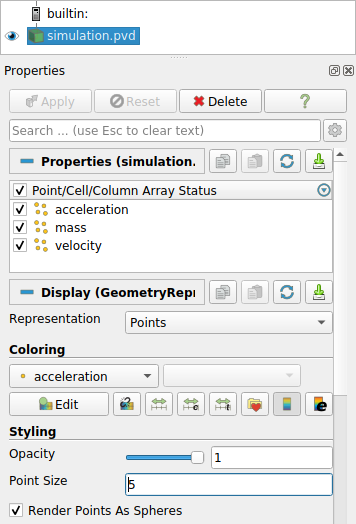
\includegraphics[width=.8\columnwidth]{figures/paraview_datapoints.png}
    \begin{tikzpicture}[overlay, scale=1.15]
      \draw[red, thick] (-3.65, 4.161) rectangle node[above right=.05cm] {\setfontsize{4pt}$2.1$ Show particles} (-2.8, 4.42);

      \draw[red, thick] (-3.65, 1.39) rectangle node[above right=.05cm and -.25cm] {\setfontsize{4pt}$2.2$ Set colors} (-1.99, 1.63);

      \draw[red, thick] (-1.6, 1.10) rectangle node[above right=.05cm and -.5cm] {\setfontsize{4pt}$2.3$ Scale colors} (-1.33, 1.34);

      \draw[red, thick] (-2.46, 1.92) rectangle node[below right=.05cm and -.425cm] {\setfontsize{4pt}$2.4$ Set representation} (-.36, 2.17);

      \draw[red, thick] (-2.46, .29) rectangle node[below right=.05cm and -.3cm] {\setfontsize{4pt}$2.5$ Set size} (-.365, .54);
    \end{tikzpicture}
  \end{column}
  \begin{column}{.61\textwidth}
    \textcolor{beamer@blendedblue}{3.} Display plot: \\[.1em]
    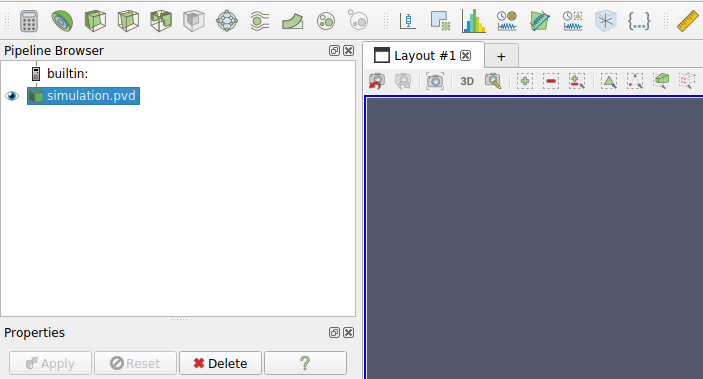
\includegraphics[width=.9\columnwidth]{figures/paraview_plot.png}
    \begin{tikzpicture}[overlay]
      \draw[red, thick] (-2.12, 3.78) rectangle node[above=.075cm] {\setfontsize{4pt}$3.1$ Create plot} (-2.42, 4.08);

      \draw[red, thick] (-7.7, 0.05) rectangle node[above right=.0125cm and .025cm] {\setfontsize{4pt}$3.2$ Show plot} (-6.81, .285);
    \end{tikzpicture} \\[.5em]
    \textcolor{beamer@blendedblue}{4.} Take screenshot:\\
    \hspace{.9em} File $\rightarrow$ Save Screenshot$\dots$ (Save All Views)

    \textcolor{beamer@blendedblue}{5.} Create animation:\\
    \hspace{.9em} File $\rightarrow$ Save Animation$\dots$ (Save All Views)
  \end{column}
\end{columns}
\end{frame}
%%%%%%%%%%%%%%%%%%%%%%%%%%%%%%%%%%%%%%%%%%%%%%%%%%%%%%%%%%%%%%%%%%%%
\begin{frame}[fragile]
  \frametitle{Submission Format}
  \begin{itemize}
    \item For each phase, \textbf{exactly} one \texttt{*.zip} or \texttt{*.tar.gz} file must be submitted in the \link{\urlIliasCourse}{ILIAS course}, containing the content corresponding to the respective phase.
    \item Phase number followed by the last names of all group members, e.g., \texttt{Phase1\_LastName1\_LastName2\_LastName3.tar.gz}.
    \item Each file must include the names of \textbf{all} contributors.
    \item Submission must be compilable and executable from the command line under Linux, i.e., \textbf{no} IDE-specific build scripts!
  \end{itemize}
\end{frame}
%%%%%%%%%%%%%%%%%%%%%%%%%%%%%%%%%%%%%%%%%%%%%%%%%%%%%%%%%%%%%%%%%%%%

%%%%%%%%%%%%%%%%%%%%%%%%%%%%%%%%%%%%%%%%%%%%%%%%%%%%%%%%%%%%%%%%%%%%
\begin{frame}[fragile]
  \frametitle{Phase 0: Formation of groups}
  \begin{itemize}
      \item Independent formation of groups of 3 members (e.g., through the \link{\urlIliasForumGroups}{ILIAS Forum}).
      \item As a \link{\urlIliasSubmissionPhaseZero}{first submission}, upload a text file with all group members and a group name for the competition in ILIAS \textbf{and} add all group members to the submission group.
      \item Deadline: \textbf{\dateDeadlinePhaseZero}
      \item If you haven't found a group by then, you must send us an email, and will be assigned to a group.
      \item If you haven't found a group by the deadline and haven't contacted us, you will \textbf{not} be considered a participant in this course!
  \end{itemize}
\end{frame}
%%%%%%%%%%%%%%%%%%%%%%%%%%%%%%%%%%%%%%%%%%%%%%%%%%%%%%%%%%%%%%%%%%%%

%%%%%%%%%%%%%%%%%%%%%%%%%%%%%%%%%%%%%%%%%%%%%%%%%%%%%%%%%%%%%%%%%%%%
\begin{frame}[fragile, c]
  \frametitle{Phase 1}
  \begin{itemize}
      \item Initial naive implementation of an n-body simulation including visualization.
      \item Simulation of two colliding galaxies with $\num{4000}$ particles.
  \end{itemize}
  \vspace*{-0.5em}
  \begin{figure}
      \centering
      \BeforeAfterImage{figures/4000_300_6000000_1_1-2_0.png}
      \hspace{1em}
      \DisplayRightArrow
      \hspace{1em}
      \BeforeAfterImage{figures/4000_300_6000000_1_1-2_6000000.png}
  \end{figure}
  \vspace*{-.5em}
  \begin{minipage}{.47\textwidth}
    \centering
    $t = \num{0}$
  \end{minipage}
  \hfill
  \begin{minipage}{.47\textwidth}
    \centering
    $t = \num{6000000}$
  \end{minipage}
\end{frame}
%%%%%%%%%%%%%%%%%%%%%%%%%%%%%%%%%%%%%%%%%%%%%%%%%%%%%%%%%%%%%%%%%%%%

%%%%%%%%%%%%%%%%%%%%%%%%%%%%%%%%%%%%%%%%%%%%%%%%%%%%%%%%%%%%%%%%%%%%
\begin{frame}[fragile, c]
  \frametitle{Phase 1: Basic idea of n-body simulations}
  The n-body simulation aims to establish motion equations for each individual particle.

  \begin{center}
  \vspace*{-1em}
  \begin{tikzpicture}
  \coordinate (origo) at (0,0.2);
  \node[below=0.1 of origo] {$(0, 0, 0)$};

  % particle 1
  \node[shading=ball,circle,minimum size=0.5cm,ball color=ForestGreen!80!white] at (5,5) (m1) {$m_1$};
  \draw [dotted,->] (origo) -- (m1) node[midway,sloped,below] {$\vec{r}_1$};
  \draw [dashed,thick,->,ForestGreen] (m1) -- ++(-1,1)  node[midway,sloped,above] {$\vec{v}_1$};
  \draw [dashed,thick,->,NavyBlue] (m1) -- ++(-0.8,-0.2) node[sloped,near end,anchor=east] {$\vec{a}_{1,2}$};
  \draw [dashed,thick,->,orange] (m1) -- ++(0.4,-0.6) node[sloped,near end,anchor=west] {$\vec{a}_{1,3}$};
  \draw [dashed,->,NavyBlue!60] (m1) ++(-1,1)  --  ++(-0.8,-0.2);
  \draw [dashed,->,orange!60] (m1) ++(-1.8,0.8)  --  ++(0.4,-0.6);
  \draw [very thick,->,red] (m1)   --  ++(-1.4,0.2);

  % particle 2
  \node[shading=ball,circle,minimum size=0.5cm,ball color=NavyBlue!80!white] at (-3,3) (m2) {$m_2$};
  \draw [dotted,->] (origo) -- (m2) node[midway,sloped,below] {$\vec{r}_2$};
  \draw [dashed,thick,->,NavyBlue] (m2) -- ++(1,1.3)  node[midway,sloped,above] {$\vec{v}_2$};
  \draw [dashed,thick,->,ForestGreen] (m2) -- ++(0.8,0.2) node[sloped,near end,anchor=west] {$\vec{a}_{2,1}$};
  \draw [dashed,thick,->,orange] (m2) -- ++(1,-0.1) node[sloped,near end,anchor=west] {$\vec{a}_{2,3}$};
  \draw [dashed,->,ForestGreen!60] (m2)++(1,1.3) -- ++(0.8,0.2);
  \draw [dashed,->,orange!60] (m2)++(1.8,1.5) -- ++(1,-0.1);
  \draw [very thick,->,red] (m2) -- ++(2.8,1.4);

  % particle 3
  \node[shading=ball,circle,minimum size=0.5cm,ball color=orange!80!white] at (7,2) (m3) {$m_3$};
  \draw [dotted,->] (origo) -- (m3) node[midway,sloped,below] {$\vec{r}_3$};
  \draw [dashed,thick,->,orange] (m3) -- ++(0.8,0.9)  node[midway,sloped,above] {$\vec{v}_3$};
  \draw [dashed,thick,->,ForestGreen] (m3) -- ++(-0.4,0.6) node[sloped,near end, anchor=east] {$\vec{a}_{3,1}$};
  \draw [dashed,thick,->,NavyBlue] (m3) -- ++(-1,0.1) node[sloped, near end, anchor=east] {$\vec{a}_{3,2}$};
  \draw [dashed,->,ForestGreen!60] (m3)++(0.8,0.9) -- ++(-0.4,0.6);
  \draw [dashed,->,NavyBlue!60] (m3)++(0.4,1.5) --  ++(-1,0.1);
  \draw [very thick,->,red] (m3) -- ++(-0.6,1.6);
  \end{tikzpicture}
  \end{center}
\end{frame}
%%%%%%%%%%%%%%%%%%%%%%%%%%%%%%%%%%%%%%%%%%%%%%%%%%%%%%%%%%%%%%%%%%%%

%%%%%%%%%%%%%%%%%%%%%%%%%%%%%%%%%%%%%%%%%%%%%%%%%%%%%%%%%%%%%%%%%%%%
\begin{frame}[fragile]
  \frametitle{Phase 1.1: Naive implementation of an n-body simulation}
    Each particle $i$ with mass $m_i$ and position vector $\vec{r}_i$ experiences the force $\vec{a}_i$ from all other particles according to Newton's law of universal gravitation:
      \begin{equation*}
        \vec{a}_i = \sum\limits_{i \neq j} G m_j \frac{\vec{r}_j - \vec{r}_i}{(\norm{\vec{r}_j - \vec{r}_i}_2^2 + \epsilon^2)^\frac{3}{2}}
      \end{equation*}
      \pause
      \begin{itemize}
        \item Gravitational constant: $G = \num{6.67428e-11}\frac{\text{m}^3}{\text{kg} \cdot \text{sec}^2}$
        \item Units do not match the given datasets:
              \begin{itemize}
                \item Mass in solar masses: $M_\odot = \SI{1.988435e30}{\kilo\gram}$
                \item Distance in parsec:  $\SI{1}{\parsec} = \SI{3.08567758129e16}{\meter}$
                \item Time in years: $\SI{1}{\year} = \num{365.25} \cdot \SI{86400}{\sec}$
              \end{itemize}
        \item Note: the correct scaling of $G$ should be calculated in the program!
        \item Softening factor: $\epsilon = 0.1$ to avoid collisions between particles
      \end{itemize}
\end{frame}
%%%%%%%%%%%%%%%%%%%%%%%%%%%%%%%%%%%%%%%%%%%%%%%%%%%%%%%%%%%%%%%%%%%%

%%%%%%%%%%%%%%%%%%%%%%%%%%%%%%%%%%%%%%%%%%%%%%%%%%%%%%%%%%%%%%%%%%%%
\begin{frame}[fragile]
  \frametitle{Phase 1.2: Energies in the system}
  \begin{itemize}
    \item Kinetic energy: $E_K = \sum\limits_{i}\frac{1}{2} m_i \norm{\vec{v}_i}_2^2$
    \item Potential energy: $E_P = -\sum\limits_{i < j} \frac{G m_i m_j}{\norm{\vec{r}_j - \vec{r}_i}_2}$
    \item Total energy in the system: $E_T = E_K + E_P$\vspace{.7em}
    \item $E_T$ remains constant in a stable simulation (energy conservation)!
  \end{itemize}
  \vfill
  \pause
  The "Virial Equilibrium":

  $$ \frac{2 \cdot E_K}{\abs{E_P}} \approx 1.0 $$

  as a dynamic equilibrium state within a timescale comparable to a multiple of the typical time it takes for a particle to traverse the system.
  \vfill
  \textbf{Question:} What happens if the result is $> 1.0$ or $< 1.0$?

  \vfill
  \setfontsize{8pt}
  See: \url{http://www.scholarpedia.org/article/n-body_simulations_(gravitational)}
\end{frame}
%%%%%%%%%%%%%%%%%%%%%%%%%%%%%%%%%%%%%%%%%%%%%%%%%%%%%%%%%%%%%%%%%%%%

%%%%%%%%%%%%%%%%%%%%%%%%%%%%%%%%%%%%%%%%%%%%%%%%%%%%%%%%%%%%%%%%%%%%
\begin{frame}[fragile]
  \frametitle{Phase 1.3: Leapfrog Method}
  The Leapfrog method, a second-order time integration method, combines two variants of the symplectic Euler method (SE) to move from time step $k$ to the next time step $k + 1$:
  \begin{equation*}
    \begin{split}
      (SE1) &\left\lbrace
      \begin{array}{rcl}
        \vec{v}^{k+\frac{1}{2}} & = & \vec{v}^k + \vec{a}^k \frac{\Delta t}{2}               \\
        \vec{r}^{k+\frac{1}{2}} & = & \vec{r}^k + \vec{v}^{k + \frac{1}{2}} \frac{\Delta t}{2}
      \end{array}\right.\\[.5em]
      (SE2) &\left\lbrace
      \begin{array}{rcl}
        \vec{r}^{k+1} & = & \vec{r}^{k + \frac{1}{2}} + \vec{v}^{k + \frac{1}{2}} \frac{\Delta t}{2} \\
        \vec{v}^{k+1} & = & \vec{v}^{k + \frac{1}{2}} + \vec{a}^{k+1} \frac{\Delta t}{2}
      \end{array}\right.\\
    \end{split}
  \end{equation*} \\
  \vfill
  \setfontsize{8pt}
  See: \texttt{O. Buneman: Time-Reversible Difference Procedures (1967)\\[-.5em]
  (DOI: \url{https://doi.org/10.1016/0021-9991(67)90056-3})}
  % https://www.sciencedirect.com/science/article/pii/0021999167900563
  % https://www.sciencedirect.com/science/article/pii/0010465587900191}
\end{frame}
%%%%%%%%%%%%%%%%%%%%%%%%%%%%%%%%%%%%%%%%%%%%%%%%%%%%%%%%%%%%%%%%%%%%

%%%%%%%%%%%%%%%%%%%%%%%%%%%%%%%%%%%%%%%%%%%%%%%%%%%%%%%%%%%%%%%%%%%%
\begin{frame}[fragile]
  \frametitle{Phase 1.4: Complete Simulation}
\begin{algorithmcl}
    \begin{algorithmic}[1]
        \State{Adjust initial velocities: $\vec{u}_i = \dfrac{\sum_j m_j \vec{v}_j}{\sum_j m_j}$;\quad$\vec{v}_i = \vec{v}_i - \vec{u}_i$}
        \State{Update accelerations $\vec{a}_i$}
        \State{Visualize initial state}
        \While{Simulation end not reached}
            \State{Perform Leapfrog time integration step}
            \If{Time step should be visualized}
                \State{Visualize time step}
            \EndIf
            \State{Update time step}
        \EndWhile
        \State{Save final state of the system as \texttt{.csv} (same format as input)}
    \end{algorithmic}
\end{algorithmcl}
\end{frame}
%%%%%%%%%%%%%%%%%%%%%%%%%%%%%%%%%%%%%%%%%%%%%%%%%%%%%%%%%%%%%%%%%%%%

%%%%%%%%%%%%%%%%%%%%%%%%%%%%%%%%%%%%%%%%%%%%%%%%%%%%%%%%%%%%%%%%%%%%
\begin{frame}[fragile]
  \frametitle{Phase 1.5: Reading the Simulation Data}
  \begin{itemize}
    \item Initial scenarios of different sizes are provided in \link{\urlIliasData}{ILIAS}: \\
        \begin{itemize}
            \item Small dataset for testing and validation: $\num{50}$ particles
            \item Medium-sized dataset for performance optimizations: $\num{500}$ particles
            \item Large dataset for final simulation: $\num{4000}$ particles
        \end{itemize}
    \item \texttt{.csv} file format: the first line contains header information, followed by the actual data:
    	\begin{minted}[bgcolor=lightgray!30]{text}
id,mass,pos_x,pos_y,pos_z,vel_x,vel_y,vel_z
0,1e+06,0,0,0,0,0,0,0
1,1.6389,5.3848,-3.9855,0.10744,1.5294e-05,2.1107e-05,0
2,5.5756,6.7128,-8.9865,0.15009,1.5936e-05,-1.2401e-05,0
	\end{minted}
    \item The values are in the following units: mass in [$M_\odot$], positions in [$\si{\parsec}$], and velocities in [$\frac{\si{\parsec}}{\si{\year}}$].
    \item Data must be stored and processed in double precision (FP64).
  \end{itemize}
\end{frame}
%%%%%%%%%%%%%%%%%%%%%%%%%%%%%%%%%%%%%%%%%%%%%%%%%%%%%%%%%%%%%%%%%%%%

%%%%%%%%%%%%%%%%%%%%%%%%%%%%%%%%%%%%%%%%%%%%%%%%%%%%%%%%%%%%%%%%%%%%
\begin{frame}[fragile]
  \frametitle{Phase 1.6: Visualization}
  Mandatory:
  \begin{itemize}
      \item Visualize the data using \link{https://www.paraview.org/}{ParaView}.
      \item Create a \texttt{.vtp} file at each visualization step, containing the current state of the simulation: particle mass, position, velocity, acceleration, and kinetic, potential, and total energy of the system.
      \item Create a single \texttt{.pvd} file for the \textbf{entire} simulation, referencing all the \texttt{.vtp} files along with their corresponding time steps.
  \end{itemize}
  \vfill
  \pause
  Optional (easier for debugging):
  \begin{itemize}
    \item Live visualization during the actual simulation.
    \item In \texttt{C++}, for example, visualize the $\dots$
    \begin{itemize}
        \item Bodies using \link{https://github.com/PointCloudLibrary/pcl}{PCL}.
        \item Energies using \link{https://github.com/lava/matplotlib-cpp}{matplotlib-cpp}.
    \end{itemize}
    \item \textbf{Important:} Other visualization libraries can be used here, but the final submission must be compilable without them.
  \end{itemize}
\end{frame}
%%%%%%%%%%%%%%%%%%%%%%%%%%%%%%%%%%%%%%%%%%%%%%%%%%%%%%%%%%%%%%%%%%%%

%%%%%%%%%%%%%%%%%%%%%%%%%%%%%%%%%%%%%%%%%%%%%%%%%%%%%%%%%%%%%%%%%%%%
\begin{frame}[fragile]
  \frametitle{Phase 1.6: Example of a \texttt{.vtp} file with 2 data points}
  \setfontsize{5.3pt}
    \begin{minted}[bgcolor=lightgray!30,obeytabs=true,tabsize=2]{xml}
<?xml version="1.0"?>
<VTKFile type="PolyData" version="0.1" byte_order="LittleEndian" header_type="UInt64">
  <PolyData>
    <Piece NumberOfPoints="2" NumberOfVerts="2">
      <Points>
        <DataArray type="Float64" Name="position" NumberOfComponents="3" format="ascii">
                    0 0 0
                    20 20 0
        </DataArray></Points>
      <PointData><DataArray type="Float64" Name="mass" NumberOfComponents="1" format="ascii">
                    1e+06
                    100000
        </DataArray>
        <!-- TODO: velocity, acceleration -->
      </PointData>
      <Verts><DataArray type="Int64" Name="offsets">
                    1 2
        </DataArray><DataArray type="Int64" Name="connectivity">
                    0 1
        </DataArray>
      </Verts>
    </Piece>
    <FieldData>
      <DataArray type="Float64" Name="kinetic energy" NumberOfTuples="1" format="ascii">
                    1.31546e-05
      </DataArray>
      <!-- TODO: potential energy, total energy -->
    </FieldData>
  </PolyData>
</VTKFile>
  \end{minted}
\end{frame}
%%%%%%%%%%%%%%%%%%%%%%%%%%%%%%%%%%%%%%%%%%%%%%%%%%%%%%%%%%%%%%%%%%%%

%%%%%%%%%%%%%%%%%%%%%%%%%%%%%%%%%%%%%%%%%%%%%%%%%%%%%%%%%%%%%%%%%%%%
\begin{frame}[fragile]
  \frametitle{Phase 1.6: Example of a \texttt{.pvd} file}
  Note: \mintinline{xml}{timestep} does not correspond to the current time step number, but to the current simulation time!
  \vfill
  Example: Time step size $dt = 0.5$ and visualization step size $vs = 10$
  \setfontsize{7.2pt}
  \begin{minted}[bgcolor=lightgray!30,obeytabs=true,tabsize=2]{xml}
<?xml version="1.0"?>
<VTKFile type="Collection" version="0.1" byte_order="LittleEndian" compressor="vtkZLibDataCompressor">
  <Collection>
    <DataSet timestep="0.0" group="" part="0" file="time_series/sim.0.vtp"/>
    <DataSet timestep="5.0" group="" part="0" file="time_series/sim.1.vtp"/>
    <DataSet timestep="10.0" group="" part="0" file="time_series/sim.2.vtp"/>
    <DataSet timestep="15.0" group="" part="0" file="time_series/sim.3.vtp"/>
  </Collection>
</VTKFile>
  \end{minted}
\end{frame}
%%%%%%%%%%%%%%%%%%%%%%%%%%%%%%%%%%%%%%%%%%%%%%%%%%%%%%%%%%%%%%%%%%%%

%%%%%%%%%%%%%%%%%%%%%%%%%%%%%%%%%%%%%%%%%%%%%%%%%%%%%%%%%%%%%%%%%%%%
\begin{frame}[fragile]
  \frametitle{Phase 1.7: Running the Simulation}

The simulation must be executable from the command line with the following parameters, which can be read in any order:
\begin{center}
    \mintinline{text}{java -jar simulate.jar --file data.csv --dt 2.5 --t_end 100.0 --vs 5}
\end{center}
Simulate every \num{2.5} years up to \num{100} years (40 time steps), with visualizations every 12.5 years (8 visualizations + the initial state).
\begin{center}
    \mintinline{text}{java -jar simulate.jar --vs 10 --dt 20 --t_end 4000 --file data2.csv}
\end{center}

\begin{description}
  \item[\texttt{--file}] the simulation file to be used
  \item[\texttt{--dt}] the time step size $\Delta t$ in years
  \item[\texttt{--t\_end}] the end time step in years
  \item[\texttt{--vs}] the visualization step size \\
  (example above: visualize every 5th or 10th time step)
\end{description}
\vfill
For \texttt{C++}, replace \mintinline{text}{java -jar simulate.jar} with \mintinline{text}{./simulate}.
\end{frame}
%%%%%%%%%%%%%%%%%%%%%%%%%%%%%%%%%%%%%%%%%%%%%%%%%%%%%%%%%%%%%%%%%%%%

%%%%%%%%%%%%%%%%%%%%%%%%%%%%%%%%%%%%%%%%%%%%%%%%%%%%%%%%%%%%%%%%%%%%
\begin{frame}[fragile]
  \frametitle{Phase 1.8: Validation of the Simulation}
    \begin{itemize}
        \item In \link{\urlIliasData}{ILIAS}, there is a \texttt{50\_ground\_truth.csv} file with the simulation result of the $\num{50}$ particle test case.
        \item Result can be reproduced with:\\
        \mintinline{text}{java -jar simulate.jar --file 50.csv --dt 100 --t_end 1000000}\\
        or\\
        \mintinline{text}{./simulate --file 50.csv --dt 100 --t_end 1000000}
        \item \textbf{Caution:} Due to floating-point inaccuracies, the results should not be tested for equality, but checked if they are sufficiently close (number of decimal places in the \texttt{.csv} file, etc.).
    \end{itemize}
\end{frame}
%%%%%%%%%%%%%%%%%%%%%%%%%%%%%%%%%%%%%%%%%%%%%%%%%%%%%%%%%%%%%%%%%%%%

%%%%%%%%%%%%%%%%%%%%%%%%%%%%%%%%%%%%%%%%%%%%%%%%%%%%%%%%%%%%%%%%%%%%
\begin{frame}[fragile, label={phase1_anforderungen}]
  \frametitle{Phase 1: Requirements}
  \vspace{.5em}
  The following simulation must not take longer than $\SI{60}{\minute}$ on the bwCloud:
  \begin{center}
    \setfontsize{10.3pt}
    \mintinline{text}{java -jar simulate.jar --file 4000.csv --dt 300 --t_end 6000000 --vs 200} \\[.75em]

    \begin{figure}
        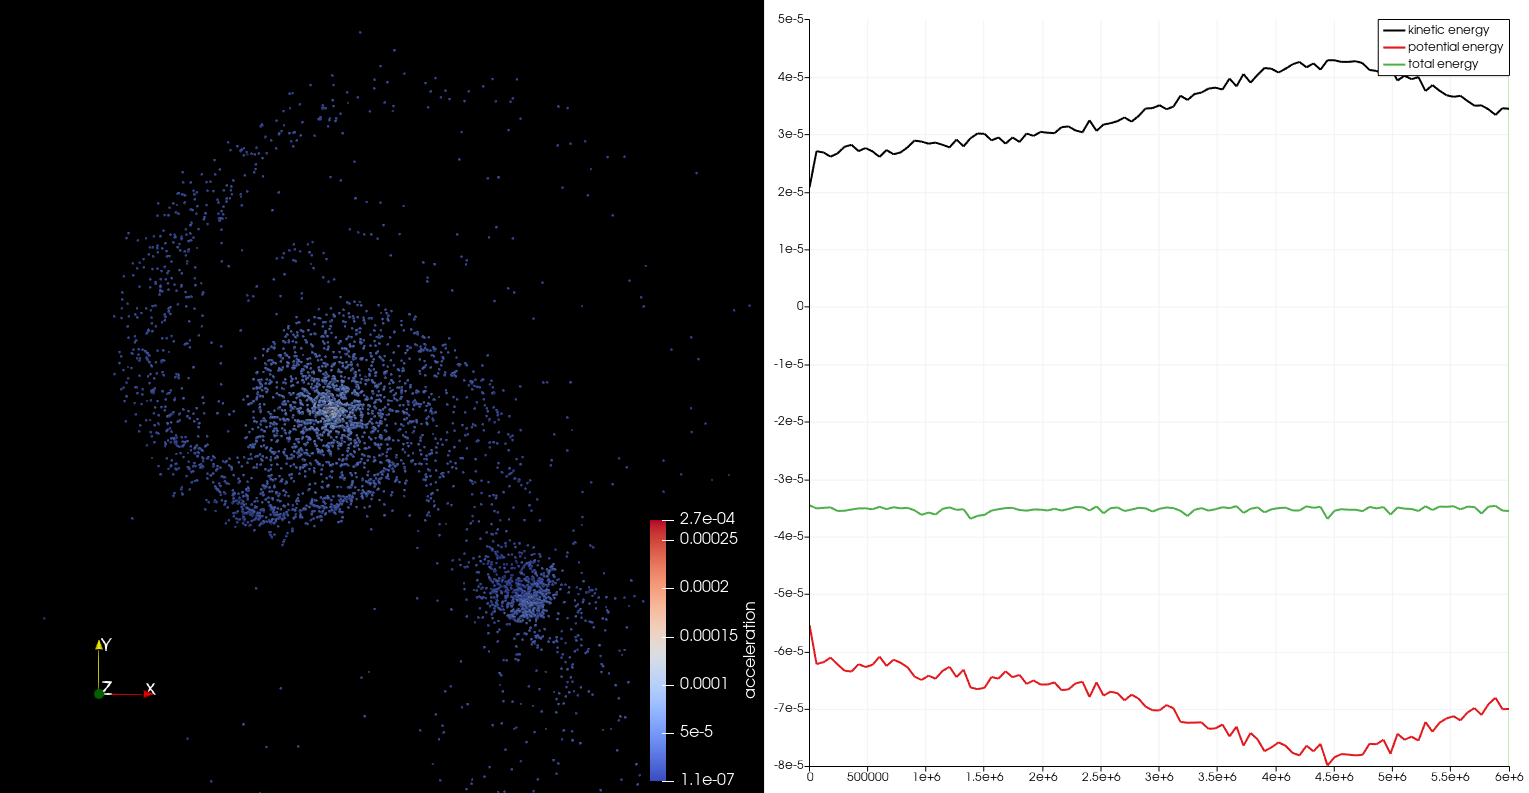
\includegraphics[width=.65\textwidth]{figures/result_phase_1.png}
        \caption{Simulation result after $\num{20000}$ time steps including energy development.}
    \end{figure}
  \end{center}
\end{frame}
%%%%%%%%%%%%%%%%%%%%%%%%%%%%%%%%%%%%%%%%%%%%%%%%%%%%%%%%%%%%%%%%%%%%

%%%%%%%%%%%%%%%%%%%%%%%%%%%%%%%%%%%%%%%%%%%%%%%%%%%%%%%%%%%%%%%%%%%%
\begin{frame}[fragile]
  \frametitle{Phase 1: Submission - \dateDeadlinePhaseOne}
  \vspace*{-1em}
  \begin{itemize}
      \item Submit via \link{\urlIliasSubmissionPhaseOne}{ILIAS}.
      \item Animation of the 3D simulation (\num{20}-\SI{30}{\second}; e.g., \link{https://trac.ffmpeg.org/wiki/How\%20to\%20speed\%20up\%20/\%20slow\%20down\%20a\%20video}{ffmpeg}) and image of the final time step created in ParaView, including an energy plot (simulation from the previous slide).
      \item A \texttt{.csv} file with the final state of the simulation.
      \item Do \textbf{not} submit the \texttt{.pvd} and \texttt{.vtp} files!
      \item Include a file \texttt{submission.sh} with the following content (replace placeholders): \vspace*{.5em}
      \begin{minted}{bash}
#!/bin/sh
git clone ${REPOSITORY_URL} ${GROUP_NAME}
cd ${GROUP_NAME} || exit
git checkout ${COMMIT_HASH}
      \end{minted}

      The commit must contain the code to be evaluated, as well as a \texttt{README} describing how to compile and run the code.
  \end{itemize}
\end{frame}
%%%%%%%%%%%%%%%%%%%%%%%%%%%%%%%%%%%%%%%%%%%%%%%%%%%%%%%%%%%%%%%%%%%%



%%%%%%%%%%%%%%%%%%%%%%%%%%%%%%%%%%%%%%%%%%%%%%%%%%%%%%%%%%%%%%%%%%%%
\begin{frame}[fragile]
  \frametitle{Phase 2:}
  
  \begin{itemize}
      \item Acceleration of the simulation using the tree-based Barnes-Hut algorithm.
      \item Simulation of the collision between the Milky Way and the Andromeda Galaxy with $\num{81920}$ particles.
  \end{itemize}
  \vspace*{0.5em}
  \begin{figure}
      \centering
      \BeforeAfterImage{figures/dubinski_0-03_120_1_1-5_0.png}
      \hspace{1em}
      \DisplayRightArrow
      \hspace{1em}
      \BeforeAfterImage{figures/dubinski_0-03_120_1_1-5_120.png}
  \end{figure}
  \begin{minipage}{.47\textwidth}
    \centering
    $t = \num{0}$
  \end{minipage}
  \hfill
  \begin{minipage}{.47\textwidth}
    \centering
    $t = \num{120}$
  \end{minipage}

  \begin{tikzpicture}[overlay]
    \node[white] at (2, 5.25) {\scriptsize Andromeda};
    \node[white] at (4.9, 2.25) {\scriptsize Milky Way};
  \end{tikzpicture}
\end{frame}
%%%%%%%%%%%%%%%%%%%%%%%%%%%%%%%%%%%%%%%%%%%%%%%%%%%%%%%%%%%%%%%%%%%%

%%%%%%%%%%%%%%%%%%%%%%%%%%%%%%%%%%%%%%%%%%%%%%%%%%%%%%%%%%%%%%%%%%%%
\begin{frame}[fragile]
  \frametitle{Phase 2.1: Barnes-Hut}
  Summary of merging particles into pseudo-particles if they are far enough apart to reduce the number of force calculations.
    \vfill
  \begin{center}
  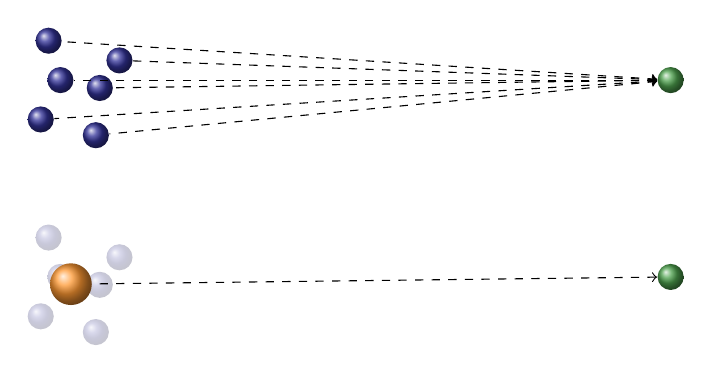
\begin{tikzpicture}
  \begin{scope}
      \node[shading=ball,circle,ball color=NavyBlue!80!white] at (0, 0) (m0) {};
      \node[shading=ball,circle,ball color=NavyBlue!80!white] at (1, 0.75) (m1) {};
      \node[shading=ball,circle,ball color=NavyBlue!80!white] at (.25, 0.5) (m2) {};
      \node[shading=ball,circle,ball color=NavyBlue!80!white] at (0.1, 1) (m3) {};
      \node[shading=ball,circle,ball color=NavyBlue!80!white] at (.75, .4) (m4) {};
      \node[shading=ball,circle,ball color=NavyBlue!80!white] at (.7, -.2) (m5) {};

      \node[shading=ball,circle,ball color=ForestGreen!80!white] at (8, .5) (mm) {};

      \foreach \x in {0,...,5}
        \draw[dashed, <-] (mm) edge (m\x);
  \end{scope}
  \begin{scope}[shift={(0, -2.5)}]
      \node[shading=ball,circle,ball color=NavyBlue!80!white,opacity=.25] at (0, 0) (m0) {};
      \node[shading=ball,circle,ball color=NavyBlue!80!white,opacity=.25] at (1, 0.75) (m1) {};
      \node[shading=ball,circle,ball color=NavyBlue!80!white,opacity=.25] at (.25, 0.5) (m2) {};
      \node[shading=ball,circle,ball color=NavyBlue!80!white,opacity=.25] at (0.1, 1) (m3) {};
      \node[shading=ball,circle,ball color=NavyBlue!80!white,opacity=.25] at (.75, .4) (m4) {};
      \node[shading=ball,circle,ball color=NavyBlue!80!white,opacity=.25] at (.7, -.2) (m5) {};

      \node[shading=ball,circle,scale=1.6,ball color=orange!80!white] at (.3833, .4083) (mcof) {};

      \node[shading=ball,circle,ball color=ForestGreen!80!white] at (8, .5) (mm) {};

      \draw[dashed, <-] (mm) edge (mcof);
  \end{scope}
  \begin{scope}[overlay]
    \draw[dotted, ->] (-.9, .4803) to [out=210,in=150] (-.9, .4803 + -2.5);
    \node[rotate=90] at (-1.8, .4803 + (-2.5 / 2) {\scriptsize Approximation};
  \end{scope}
  \end{tikzpicture}
  \end{center}
  \vfill
  \setfontsize{8pt}
  See: \texttt{Josh Barnes and Piet Hut: A hierarchical O(N log N) force-calculation algorithm (1986)\\[-.5em]
  (DOI: \url{https://doi.org/10.1038/324446a0})}
\end{frame}
%%%%%%%%%%%%%%%%%%%%%%%%%%%%%%%%%%%%%%%%%%%%%%%%%%%%%%%%%%%%%%%%%%%%

%%%%%%%%%%%%%%%%%%%%%%%%%%%%%%%%%%%%%%%%%%%%%%%%%%%%%%%%%%%%%%%%%%%%
\begin{frame}[fragile]
  \frametitle{Theory: Barnes-Hut - Example: Quadtree}
  \begin{tikzpicture}
    \begin{scope}[scale=0.9]
        % Quadtree grid
        \draw[step=4] (0, 0) grid (8, 8);
        
        \draw[step=2] (0, 0) grid (4, 4);
        \draw[step=2] (4, 4) grid (8, 8);
        \draw[step=2] (4, 0) grid (8, 4);
        
        \draw[step=1] (0, 0) grid (2, 2);
        \draw[step=1] (0, 2) grid (2, 4);
        \draw[step=1] (2, 0) grid (4, 2);
        \draw[step=1] (4, 4) grid (6, 6);
        \draw[step=1] (6, 4) grid (8, 6);
        
        \draw[thick,orange] (0, 0) rectangle (4, 4);
        
        
        % bodies
        % top left
        
        % top right
        % 1.337
        \node[shading=ball,circle,ball color=NavyBlue!80!white] (p1) at (4.35, 4.4) {};
        \node[shading=ball,circle,ball color=NavyBlue!80!white] (p2) at (4.5, 5.4) {};
        \node[shading=ball,circle,ball color=NavyBlue!80!white] (p3) at (5.6, 4.7) {};
        
        \node[shading=ball,circle,ball color=ForestGreen!80!white] (p) at (6.3, 4.65) {};
        \node[shading=ball,circle,ball color=NavyBlue!80!white] (p4) at (6.4, 5.25) {};
        \node[shading=ball,circle,ball color=NavyBlue!80!white] (p5) at (7.5, 7.5) {};
        
        % bottom left
        \node[shading=ball,circle,ball color=NavyBlue!80!white,opacity=.25] at (1.5, 1.5) {};
        \node[shading=ball,circle,ball color=NavyBlue!80!white,opacity=.25] at (0.6, 0.7) {};
        \node[shading=ball,circle,ball color=NavyBlue!80!white,opacity=.25] at (1.4, 2.3) {};
        \node[shading=ball,circle,ball color=NavyBlue!80!white,opacity=.25] at (0.75, 2.4) {};
        \node[shading=ball,circle,ball color=NavyBlue!80!white,opacity=.25] at (1.3, 0.75) {};
        \node[shading=ball,circle,ball color=NavyBlue!80!white,opacity=.25] at (2.22, 0.78) {};
        \node[shading=ball,circle,ball color=NavyBlue!80!white,opacity=.25] at (2.4, 1.3) {};
        
        % center of mass of distant bodies
        \node[shading=ball,circle,scale=1.7,ball color=orange!80!white] (pp) at (1.45, 1.39) {}; % 0.6844
        
        % bottom right % 1.821
        \node[shading=ball,circle,ball color=NavyBlue!80!white] (p6) at (7.5, 1.75) {}; % 0.637
        \node[shading=ball,circle,ball color=NavyBlue!80!white] (p7) at (6.8, 3.5) {}; % 1.594
        
        
        % theta
        \draw[thick,dashed,<-] (p) -- (pp) node[midway, pos=.3, below] {$\vec{d}$};
        \draw [decorate,decoration={brace,amplitude=10pt,raise=4pt}] (0.01, 4) -- (3.99, 4) node [midway,yshift=.7cm] {\small edge length};
        \foreach \x in {1,...,7}
            \draw[dotted,<-] (p) -- (p\x);
    \end{scope}
    
    \begin{scope}[overlay, scale=0.9]
        \node[align=left,text width=5cm] (nt) at (12.5, 7.5) {Use pseudo-particles to calculate the forces if:};
        \node[align=center, below=-.1cm of nt] {$\dfrac{\text{edge length}}{\norm{\vec{d}}_2} < \theta$};
    \end{scope}
    \begin{scope}[shift={(8, -1.5)}, scale=0.95]
        \node[shading=ball,circle,scale=2.5,ball color=orange!80!white,opacity=.25] (root) at (3.1, 6) {};
        
        % top right
        \node[shading=ball,circle,scale=1.6,ball color=orange!80!white,opacity=.25] (l11) at (1, 5) {};
        \node[shading=ball,circle,ball color=NavyBlue!80!white] (l21) at (0.3, 4) {};
        \node[shading=ball,circle,scale=1.2,ball color=orange!80!white,opacity=.25] (l22) at (1, 4) {};
        \node[shading=ball,circle,ball color=NavyBlue!80!white] (l31) at (0.8, 3) {};
        \node[shading=ball,circle,ball color=ForestGreen!80!white] (l32) at (1.2, 3) {};
        \node[shading=ball,circle,scale=1.3,ball color=orange!80!white,opacity=.25] (l23) at (2, 4) {};
        \node[shading=ball,circle,ball color=NavyBlue!80!white] (l33) at (1.6, 3) {};
        \node[shading=ball,circle,ball color=NavyBlue!80!white] (l34) at (2, 3) {};
        \node[shading=ball,circle,ball color=NavyBlue!80!white] (l35) at (2.4, 3) {};
        
        \draw[thick] (root) -- (l11);
        \draw[thick] (l11) -- (l21);
        \draw[thick] (l11) -- (l22);
        \draw[thick] (l11) -- (l23);
        \draw[thick] (l22) -- (l31);
        \draw[thick] (l22) -- (l32);
        \draw[thick] (l23) -- (l33);
        \draw[thick] (l23) -- (l34);
        \draw[thick] (l23) -- (l35);
        
        % bottom right
        \node[shading=ball,circle,scale=1.2,ball color=orange!80!white,opacity=.25] (l12) at (3.1, 5) {};
        \node[shading=ball,circle,ball color=NavyBlue!80!white] (l24) at (2.8, 4) {};
        \node[shading=ball,circle,ball color=NavyBlue!80!white] (l25) at (3.4, 4) {};
        \draw[thick] (root) -- (l12);
        \draw[thick] (l12) -- (l24);
        \draw[thick] (l12) -- (l25);
        
        % bottom left
        \node[shading=ball,circle,scale=1.7,ball color=orange!80!white] (l13) at (5.2, 5) {};
        \node[shading=ball,circle,scale=1.2,ball color=orange!80!white,opacity=.25] (l26) at (4.2, 4) {};
        \node[shading=ball,circle,ball color=NavyBlue!80!white,opacity=.25] (l36) at (4.4, 3) {};
        \node[shading=ball,circle,ball color=NavyBlue!80!white,opacity=.25] (l37) at (4, 3) {};
        \node[shading=ball,circle,scale=1.3,ball color=orange!80!white,opacity=.25] (l27) at (5.2, 4) {};
        \node[shading=ball,circle,ball color=NavyBlue!80!white,opacity=.25] (l38) at (4.8, 3) {};
        \node[shading=ball,circle,ball color=NavyBlue!80!white,opacity=.25] (l39) at (5.2, 3) {};
        \node[shading=ball,circle,ball color=NavyBlue!80!white,opacity=.25] (l310) at (5.6, 3) {};
        \node[shading=ball,circle,scale=1.2,ball color=orange!80!white,opacity=.25] (l28) at (6.2, 4) {};
        \node[shading=ball,circle,ball color=NavyBlue!80!white,opacity=.25] (l311) at (6, 3) {};
        \node[shading=ball,circle,ball color=NavyBlue!80!white,opacity=.25] (l312) at (6.4, 3) {};
        \draw[thick] (root) -- (l13);
        \draw[thick,opacity=.25] (l13) -- (l26);
        \draw[thick,opacity=.25] (l13) -- (l27);
        \draw[thick,opacity=.25] (l13) -- (l28);
        \draw[thick,opacity=.25] (l26) -- (l36);
        \draw[thick,opacity=.25] (l26) -- (l37);
        \draw[thick,opacity=.25] (l27) -- (l38);
        \draw[thick,opacity=.25] (l27) -- (l39);
        \draw[thick,opacity=.25] (l27) -- (l310);
        \draw[thick,opacity=.25] (l28) -- (l311);
        \draw[thick,opacity=.25] (l28) -- (l312);
        
        \node[anchor=west] at (0, 2.2) {\small naive: $\num{14}$ force calculations};
        \node[anchor=west] at (0, 1.7) {\small Barnes-Hut: $\num{8}$ force calculations};
    \end{scope}
  \end{tikzpicture}
\end{frame}
%%%%%%%%%%%%%%%%%%%%%%%%%%%%%%%%%%%%%%%%%%%%%%%%%%%%%%%%%%%%%%%%%%%%

%%%%%%%%%%%%%%%%%%%%%%%%%%%%%%%%%%%%%%%%%%%%%%%%%%%%%%%%%%%%%%%%%%%%
\begin{frame}[fragile]
  \frametitle{Phase 2.3: Barnes-Hut - Nodes}
  Each tree node of the octree (extension of the quadtree for $3$-dimensional space) must store the following values:
  \begin{itemize}
      \item Edge length of the octree octant
      \item Total mass of all particles in the octant: $m_{oct} = \sum_i m_i$
      \item Center of mass of all particles $i$ in the octant: $\vec{c}_{oct} = \dfrac{\sum_i m_i \vec{r}_i}{\sum_i m_i}$
      \item All children of the octant
  \end{itemize}
  \vfill
  Each octree leaf can contain at most one particle!
\end{frame}
%%%%%%%%%%%%%%%%%%%%%%%%%%%%%%%%%%%%%%%%%%%%%%%%%%%%%%%%%%%%%%%%%%%%

%%%%%%%%%%%%%%%%%%%%%%%%%%%%%%%%%%%%%%%%%%%%%%%%%%%%%%%%%%%%%%%%%%%%
\begin{frame}[fragile]
  \frametitle{Phase 2.4: Barnes-Hut - Updating Accelerations $\vec{a}_i$}
  \begin{algorithmcl}
    \begin{algorithmic}[1]
        \Procedure{UpdateAcceleration}{\texttt{Particle}, \texttt{Node}}
        \State{Calculate direction vector $\vec{d}$ between \texttt{Particle} and \texttt{Node}}
        \If{Pseudo-particle can be used $\vee$ \texttt{Node} is a leaf node}
                    \State{Update acceleration of $\vec{a}_\text{\texttt{particle}}$}
                \Else
                    \For{each \texttt{Child$_i$} of \texttt{Node}}
                        \State{\textsc{UpdateAcceleration}(\texttt{Particle}, \texttt{child}$_i$)}
                    \EndFor
                \EndIf
                \EndProcedure
    \end{algorithmic}
    \end{algorithmcl}
    \vfill
    \textbf{Question:} \\
    Can the energy calculation also be accelerated using the Barnes-Hut tree?
\end{frame}
%%%%%%%%%%%%%%%%%%%%%%%%%%%%%%%%%%%%%%%%%%%%%%%%%%%%%%%%%%%%%%%%%%%%

%%%%%%%%%%%%%%%%%%%%%%%%%%%%%%%%%%%%%%%%%%%%%%%%%%%%%%%%%%%%%%%%%%%%
\begin{frame}[fragile]
    \frametitle{Phase 2.5: Running the Simulation}

    The simulation must be executable from the command line as follows:
    \begin{minted}[breaklines=true]{text}
java -jar simulate.jar --file data.csv --dt 2.0 --t_end 100.0 --vs 5 --algorithm_type 1 --theta 1.5
    \end{minted}

    \begin{description}[labelwidth=\widthof{\bfseries \texttt{--theta}}]
        \item[\texttt{--file}] the simulation file to be used
        \item[\texttt{--dt}] the time step size $\Delta t$ in years
        \item[\texttt{--t\_end}] the end time step in years
        \item[\texttt{--vs}] the visualization step size
        \item[\texttt{--algorithm\_type}] the algorithm to be used \\
        (0: naive brute-force algorithm; 1: Barnes-Hut algorithm)
        \item[\texttt{--theta}] the threshold in the Barnes-Hut algorithm
    \end{description}
    \vfill
    For \texttt{C++}, replace \mintinline{text}{java -jar simulate.jar} with \mintinline{text}{./simulate}.
\end{frame}
%%%%%%%%%%%%%%%%%%%%%%%%%%%%%%%%%%%%%%%%%%%%%%%%%%%%%%%%%%%%%%%%%%%%

%%%%%%%%%%%%%%%%%%%%%%%%%%%%%%%%%%%%%%%%%%%%%%%%%%%%%%%%%%%%%%%%%%%%
\begin{frame}[fragile]
    \frametitle{Phase 2.6: Performance Analysis}
    \begin{itemize}
    \item A scaling plot (double logarithmic axis scaling; $x$-axis: number of particles, $y$-axis: runtime) with varying number of particles for the naive algorithm and Barnes-Hut.
    \item Landau complexity estimation ($\mathcal{O}$ notation) of your own code based on the scaling plot.
    \item A plot that compares different $\theta$ values in the Barnes-Hut algorithm ($x$-axis) with their runtime ($y_1$-axis) and error (sum of Euclidean distances compared to the naive approach) ($y_2$-axis).
    \item Explanations with \textbf{justifications} for both plots!
    \item \textbf{Note:} Come up with suitable scenarios for both plots.
    \end{itemize}
    % https://thesis.library.caltech.edu/6291/ (page 83)
\end{frame}
%%%%%%%%%%%%%%%%%%%%%%%%%%%%%%%%%%%%%%%%%%%%%%%%%%%%%%%%%%%%%%%%%%%%

%%%%%%%%%%%%%%%%%%%%%%%%%%%%%%%%%%%%%%%%%%%%%%%%%%%%%%%%%%%%%%%%%%%%
% @helium: /import/www.ipvs/IPVS/SC/cgi-bin/n-body
%
\begin{frame}[fragile]
    \frametitle{Phase 2.6: Performance Analysis - Dataset Generation}

    Datasets with $\num{2}$ to $\num{200000}$ particles can be generated using a \mintinline{bash}{wget} or \mintinline{bash}{curl} call (exemplary with $\num{200}$ particles):

    {
        \setfontsize{7.7pt}
        \begin{minted}[breaklines=true]{bash}
wget --user ${USERNAME} --ask-password "https://ipvs.informatik.uni-stuttgart.de/SC/cgi-bin/n-body/generate.php/?num_particles=200" -O data.csv
        \end{minted}
        \vspace*{-2em}
        \begin{minted}[breaklines=true]{bash}
curl --user ${USERNAME} "https://ipvs.informatik.uni-stuttgart.de/SC/cgi-bin/n-body/generate.php/?num_particles=200" -o data.csv
        \end{minted}
    }

    Your username corresponds to the group name from Phase 0, and you will receive the randomly generated password from us after passing Phase 1.
    % https://www.redim.de/blog/passwortschutz-mit-htaccess-einrichten
\end{frame}
%%%%%%%%%%%%%%%%%%%%%%%%%%%%%%%%%%%%%%%%%%%%%%%%%%%%%%%%%%%%%%%%%%%%

%%%%%%%%%%%%%%%%%%%%%%%%%%%%%%%%%%%%%%%%%%%%%%%%%%%%%%%%%%%%%%%%%%%%
\begin{frame}[fragile]
    \frametitle{Phase 2: Requirements}
    
    The following simulations must not take longer than $\SI{60}{\minute}$ on the bwCloud:
    \vspace*{-.5em}
    \begin{center}
    \setfontsize{7pt}
    \begin{minted}{bash}
java -jar simulate.jar --file 20000.csv --dt 300 --t_end 6000000 --vs 200 --algorithm_type 1 --theta 1.2
java -jar simulate.jar --file dubinski.csv --dt 0.03 --t_end 120.0 --vs 20 --algorithm_type 1 --theta 1.5
    \end{minted}
    \vspace*{-1.5em}
    \begin{figure}
        \captionsetup{justification=centering}
        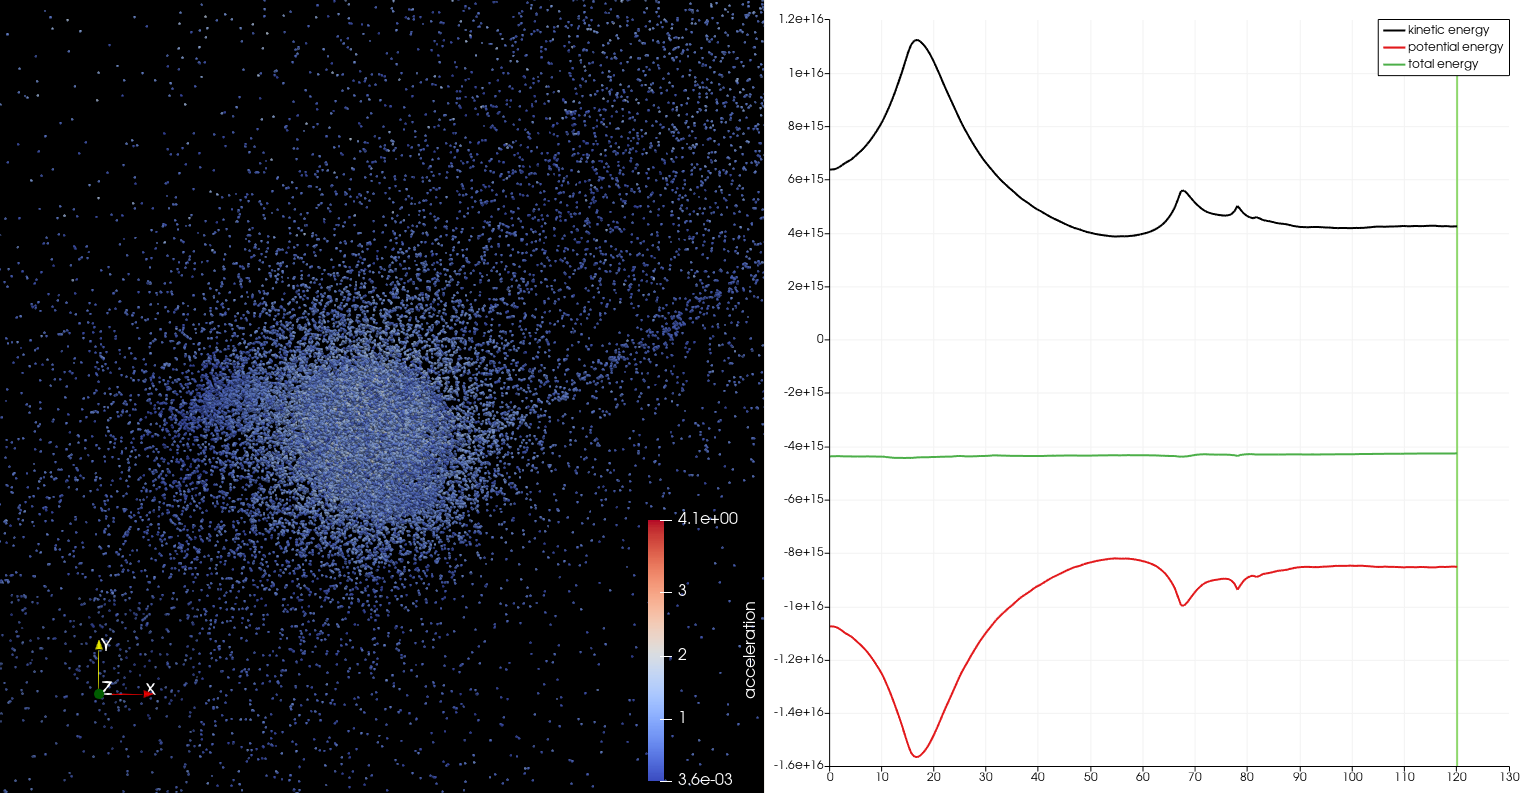
\includegraphics[width=.65\textwidth]{figures/result_phase_2.png}
        \caption{Simulation result of the Dubinski dataset after $\num{4000}$ time steps including energy development.}
    \end{figure}
    \end{center}
\end{frame}
%%%%%%%%%%%%%%%%%%%%%%%%%%%%%%%%%%%%%%%%%%%%%%%%%%%%%%%%%%%%%%%%%%%%

%%%%%%%%%%%%%%%%%%%%%%%%%%%%%%%%%%%%%%%%%%%%%%%%%%%%%%%%%%%%%%%%%%%%
\begin{frame}[fragile]
    \frametitle{Phase 2: Submission - \dateDeadlinePhaseTwo}
    \begin{itemize}
        \item Submission via \link{\urlIliasSubmissionPhaseTwo}{ILIAS}.
        \item Animations of the 3D simulations (each \num{20}-\SI{30}{\second}; e.g., \link{https://trac.ffmpeg.org/wiki/How\%20to\%20speed\%20up\%20/\%20slow\%20down\%20a\%20video}{ffmpeg}) and images of the final time steps created in ParaView, including the respective energy plot (simulations from previous slide).
        \item \texttt{.csv} files with the final states of the simulations.
        \item Do \textbf{not} submit the \texttt{.pvd} and \texttt{.vtp} files!
        \item A file \texttt{submission.sh} with the same content as in \hyperref[phase1_anforderungen]{Phase 1} with the \textbf{adjusted} commit hash.
        \item Double logarithmic scaling plot \textbf{including justification} of the Landau complexities.
        \item Plot of the runtime behavior and accuracy of the Barnes-Hut algorithm with different $\theta$ values \textbf{including justification} of the behavior.
    \end{itemize}
\end{frame}
%%%%%%%%%%%%%%%%%%%%%%%%%%%%%%%%%%%%%%%%%%%%%%%%%%%%%%%%%%%%%%%%%%%%

%%%%%%%%%%%%%%%%%%%%%%%%%%%%%%%%%%%%%%%%%%%%%%%%%%%%%%%%%%%%%%%%%%%%
\begin{frame}[fragile]
    \frametitle{Conclusion}
    \begin{itemize}
    \item Presentation max. $\SI{5}{\minute}$ per group.
    \item One slide with challenges you encountered.
    \item One slide each with the plots required in Phase 2.
    \item Slides must also be uploaded to \link{\urlIliasSubmissionFinal}{ILIAS}.
    \item Explanation of the plots, for example, based on your own code.
    \item Each group member must be able to answer questions about their own code!
    \end{itemize}
\end{frame}
%%%%%%%%%%%%%%%%%%%%%%%%%%%%%%%%%%%%%%%%%%%%%%%%%%%%%%%%%%%%%%%%%%%%


%%%%%%%%%%%%%%%%%%%%%%%%%%%%%%%%%%%%%%%%%%%%%%%%%%%%%%%%%%%%%%%%%%%%
\begin{frame}[fragile]
    \frametitle{Competition - Who is the Fastest?}
    \begin{itemize}
        \item Runtimes for the submissions of both phases.
        \item Enter your current runtimes (in seconds) in a table: \\
        Table: {\setfontsize{9pt}\url{\urlNextcloud}} \\
        Password: \texttt{\passwordNextcloud}
        \item Runtimes do not have to be entered only at the end but can be updated.
        \item The runtimes will be verified by us at the end.
        \item Real simulation without tricks (e.g., outputting pre-calculated time steps is \textbf{not} allowed)!
        \item The fastest group will receive a small prize.
    \end{itemize}
\end{frame}
%%%%%%%%%%%%%%%%%%%%%%%%%%%%%%%%%%%%%%%%%%%%%%%%%%%%%%%%%%%%%%%%%%%%

%%%%%%%%%%%%%%%%%%%%%%%%%%%%%%%%%%%%%%%%%%%%%%%%%%%%%%%%%%%%%%%%%%%%
\begin{frame}[fragile]
    \frametitle{General Recommendations - 1}
    \begin{itemize}
    \item Your simulation should have a progress indicator (e.g., console output every \SI{10}{\percent} of the simulation).
    \item Use an IDE (Visual Studio Code, CLion, Eclipse, IntelliJ, etc.) and its features such as profilers, debuggers, auto-formatting, linters, etc.
    \item Use an automated build system like CMake or Maven.
    \item Document your code (for us \textbf{and} for yourself!) using tools like \link{https://doxygen.nl/}{Doxygen}/\link{https://www.oracle.com/java/technologies/javase/javadoc-tool.html}{JavaDoc}.
    \item Make the installation, usage of your program, and verification of the requirements as easy as possible for the user.
    \item Test your program on the target system, the bwCloud (it must be runnable on Linux (keyword: paths: \mintinline{text}{/} vs \mintinline{text}{\})!).
    \item Questions can be asked directly in the \link{\urlIliasForumGeneral}{ILIAS forum}.
    \end{itemize}
\end{frame}

\begin{frame}[fragile]
    \frametitle{General Recommendations - 2}
    \begin{itemize}
    \item For \textbf{Windows users}, to avoid headaches due to different line endings on Linux and Windows, use\link{https://docs.github.com/en/get-started/getting-started-with-git/configuring-git-to-handle-line-endings}{}:
    \mintinline{text}{git config --global core.autocrlf true}
    \item If you are using \texttt{C++}: objects allocated with \mintinline{c++}{new} are \textbf{not} automatically released (better: use \mintinline{c++}{std::unique_ptr/std::shared_ptr} if necessary)!
    \item If you are using Java, avoid \enquote{boxed types} as much as possible:\\
    \mintinline{java}{double} vs. \mintinline{java}{Double} or \mintinline{java}{double[]} vs. \mintinline{java}{ArrayList<Double>}!
    \item Another tip for Java users: avoid using \mintinline{java}{Math.pow} in performance-critical code!
%     \item Another tip for Java users:
%     \begin{minted}[escapeinside=||,mathescape=true]{java}
% final double x = |$\dots$|;
% final double r = Math.pow(x, -2.5);
%     \end{minted}
%     is significantly slower in Java (for unclear reasons) than
%     \begin{minted}[escapeinside=||,mathescape=true]{java}
% final double x = |$\dots$|;
% final double r = 1.0 / Math.sqrt(x * x * x * x * x);
%     \end{minted}
    \item The runtime of your own code can be determined most easily using \mintinline{bash}{time}: \\[-.7em]
    {
        \small
        \begin{minted}{bash}
time java -jar simulate.jar --file data.csv --dt 10 --t_end 100 --vs 2
        \end{minted}
    }%
    \vspace*{-1.75em}
    \item If only an IPv6 address is available on the bwCloud, use \texttt{mvn -Djava.net.preferIPv6Addresses=true package} to build your Java programs. 
    \item In the Barnes-Hut algorithm, pay attention that the large black hole isn't located at the intersection point of all eight quadrants. 
    \item MIT insider tip: \link{https://missing.csail.mit.edu/}{\enquote{The Missing Semester of Your CS Education}}
    \end{itemize}
\end{frame}
%%%%%%%%%%%%%%%%%%%%%%%%%%%%%%%%%%%%%%%%%%%%%%%%%%%%%%%%%%%%%%%%%%%%


%%%%%%%%%%%%%%%%%%%%%%%%%%%%%%%%%%%%%%%%%%%%%%%%%%%%%%%%%%%%%%%%%%%%
\begin{frame}
  \frametitle{Important Dates}
  \begin{description}
    \item[\dateKickoffPhaseOne] Kick-off
    \item[\dateDeadlinePhaseZero] Group formation deadline
    \item[\dateKickoffPhaseTwo] Kick-off Phase 2
    \item[\dateDeadlinePhaseOne] Phase 1 deadline
    \item[\dateDeadlinePhaseTwo] Phase 2 deadline
    \item[\dateFinal] Final presentations% (possibly multiple dates)
  \end{description}
  \vspace{1cm}
  \pause
  \DisplayRightArrow\quad Don't forget to register in \link{https://campus.uni-stuttgart.de}{C@MPUS}!
\end{frame}
%%%%%%%%%%%%%%%%%%%%%%%%%%%%%%%%%%%%%%%%%%%%%%%%%%%%%%%%%%%%%%%%%%%%
